\documentclass[11pt,a4paper]{report}

% Latin Modern must come before microtype. Under T1 the default Computer Modern
% resolves to bitmap fonts, and microtype's font expansion is only possible with
% scalable ones, which pdfTeX reports as a fatal error rather than a warning.
\usepackage{lmodern}
\usepackage[T1]{fontenc}
\usepackage[utf8]{inputenc}
\usepackage[margin=2.6cm]{geometry}
\usepackage{amsmath}
\usepackage{amssymb}
\usepackage{booktabs}
\usepackage{graphicx}
\usepackage{microtype}
\usepackage{siunitx}
\usepackage{xcolor}
\usepackage{listings}
\usepackage{caption}
\usepackage[hidelinks]{hyperref}

\sisetup{group-separator={,}, group-minimum-digits=4}

\definecolor{codebg}{HTML}{F5F5F2}
\definecolor{rule}{HTML}{C3C2B7}
\lstset{
  basicstyle=\ttfamily\footnotesize,
  backgroundcolor=\color{codebg},
  frame=single,
  rulecolor=\color{rule},
  breaklines=true,
  columns=fullflexible,
  showstringspaces=false,
  captionpos=b
}

\captionsetup{font=small, labelfont=bf}

% Measured values, generated by scripts/gen_report_assets.py from the recorded
% results. Nothing in the prose of this report is a number typed by hand.
% Generated by scripts/gen_report_assets.py. Do not edit by hand.
% Every value here comes from a file written by a run.
\newcommand{\AllGatesPass}{true}
\newcommand{\BenchCommit}{8e4c710216be}
\newcommand{\BenchFastMath}{on}
\newcommand{\BenchSeed}{20260802}
\newcommand{\BenchTimestamp}{2026-08-02T20:11:14Z}
\newcommand{\BestTileMs}{11.842}
\newcommand{\BestTileWidth}{256}
\newcommand{\CudaRuntime}{13.3}
\newcommand{\EnergyDriftMeasured}{$1.33 \times 10^{-5}$}
\newcommand{\FusedMsAtMaxN}{45.72}
\newcommand{\FusionCeilingMs}{0.0087}
\newcommand{\FusionCeilingPercent}{0.019}
\newcommand{\FusionGainPercentAtMaxN}{+0.1}
\newcommand{\FusionGainPercentAtMinN}{+2.1}
\newcommand{\FusionSpeedupAtMaxN}{1.001}
\newcommand{\GateCount}{10}
\newcommand{\GpuBandwidthEfficiency}{81.8}
\newcommand{\GpuBusBits}{192}
\newcommand{\GpuCompute}{12.0}
\newcommand{\GpuMeasuredBandwidth}{549.9}
\newcommand{\GpuName}{NVIDIA GeForce RTX 5070}
\newcommand{\GpuPeakBandwidth}{672.0}
\newcommand{\GpuSms}{48}
\newcommand{\LadderMaxN}{200,000}
\newcommand{\LadderMinN}{10,000}
\newcommand{\LsuReduction}{3.8}
\newcommand{\MeasuredFlopsPerInteraction}{18.0}
\newcommand{\MomentumDriftMeasured}{$1.23 \times 10^{-8}$}
\newcommand{\NaiveDramPct}{0.55}
\newcommand{\NaiveIssuePct}{50.1}
\newcommand{\NaiveLoneTexPct}{80.2}
\newcommand{\NaiveMsAtMaxN}{88.27}
\newcommand{\PeakTflops}{17.50}
\newcommand{\PlummerPValue}{0.4416}
\newcommand{\PolySixNormalisationError}{$6.48 \times 10^{-8}$}
\newcommand{\SectorReduction}{63.8}
\newcommand{\SpecifiedTileMs}{12.658}
\newcommand{\SphDensityErrorPercent}{4.20}
\newcommand{\SphFpsAtFiftyThousand}{2,963}
\newcommand{\SphFpsAtMaxN}{1,693}
\newcommand{\SphMaxN}{100,000}
\newcommand{\SphMsAtFiftyThousand}{0.337}
\newcommand{\SphMsAtMaxN}{0.591}
\newcommand{\TileWidthGainPercent}{6.4}
\newcommand{\TiledDramPct}{0.45}
\newcommand{\TiledIssuePct}{74.5}
\newcommand{\TiledLoneTexPct}{39.9}
\newcommand{\TiledMsAtMaxN}{45.78}
\newcommand{\TiledTflopsAtMaxN}{17.47}
\newcommand{\TilingSpeedupAtMaxN}{1.93}


\title{\textbf{Particle Physics Simulation}\\[0.4em]
       \large Measuring what the memory hierarchy is worth, and proving the
       physics is right}
\author{Olajide Badejo}
\date{August 2026}

\begin{document}

\maketitle

\begin{abstract}
\noindent
This report describes a CUDA particle physics engine that solves two problems:
direct all pairs gravitational N-body dynamics, and weakly compressible
smoothed particle hydrodynamics with spatial hash neighbour search. It is built
around two commitments. Every optimisation is a measured result rather than a
claim, and physical correctness is enforced by conservation tests rather than
by how the output looks.

The N-body force kernel exists in three variants that isolate one technique
each. On an RTX 5070 at \LadderMaxN{} particles, shared memory tiling takes the
step from \NaiveMsAtMaxN{} to \TiledMsAtMaxN{} milliseconds, a factor of
\TilingSpeedupAtMaxN{}, and sustains \TiledTflopsAtMaxN{} TFLOP/s of single
precision arithmetic. Fusing the force evaluation with the integrator, which
was expected beforehand to be worth ten to twenty percent, is worth
\FusionGainPercentAtMaxN{} percent. That gap is not a disappointing result; it
is the most informative one in the report, and Section~\ref{sec:fusion}
explains why an arithmetic bound problem cannot be helped by removing memory
traffic, using hardware counters that put device memory throughput below one
percent of peak for all three variants.

All \GateCount{} physics gates pass. A two body circular orbit conserves energy
to \EnergyDriftMeasured{} over ten thousand velocity Verlet steps against a
limit of one part in a thousand; total momentum in a ten thousand particle
Plummer sphere holds to \MomentumDriftMeasured{}; the sampled radial density of
that sphere matches the analytic Plummer profile at a chi squared p value of
\PlummerPValue{}. The fluid solver runs \SphMaxN{} particles at
\SphMsAtMaxN{} milliseconds per step.
\end{abstract}

\tableofcontents

\chapter{Introduction}

\section{What this is}

This is a particle physics engine written in CUDA. It solves two problems that
sit at opposite ends of the memory access spectrum, which is the reason both
are here.

The first is direct all pairs gravitational N-body dynamics. Every particle
attracts every other, so the force evaluation is $O(N^2)$ arithmetic over $O(N)$
data. Access is perfectly regular and entirely predictable.

The second is smoothed particle hydrodynamics, in which a particle interacts
only with the neighbours inside a finite smoothing radius. The work is nearly
linear in the particle count, but which particles are neighbours changes every
step and has to be discovered before any physics can be evaluated. Access is
irregular and data dependent.

A GPU rewards the first pattern and punishes the second, and the techniques
that matter are different in each case. Putting both in one engine, behind one
configuration format and one integrator, makes the contrast concrete.

\section{The two commitments}

\paragraph{No number without a run.} Every performance figure in this report
was produced by a program in this repository, recorded to a comma separated
file with the commit that produced it, and read back into this document
mechanically. The only typed values are \texttt{v1.0.0} values in correction records and
a few figures from one off runs that no file records, such as the double precision
truncation error in Section~\ref{sec:gates}. Where I had an expectation
before measuring, the expectation is stated and then compared with what
actually happened. Where a published claim turned out to be wrong,
Chapter~\ref{ch:corrections} says so.

\paragraph{Correctness is enforced, not observed.} A particle simulation that
is subtly wrong still looks like a particle simulation. Fluid still sloshes and
stars still orbit when the force law has a sign error in one term or the
neighbour search quietly counts some particles twice. The defence is a set of
conservation and distribution tests with numerical thresholds, run by the test suite on
a machine with a GPU, that fail loudly. There are \GateCount{} of them and
Chapter~\ref{ch:results} reports what each one measured.

These two commitments interact. The benchmark builds use \texttt{fast math},
which lowers the reciprocal square root to a hardware approximation. The physics gates
should not depend on a flag like that. So the build compiles the device library twice from
identical sources, once with fast math for the benchmarks and once without for
the gates. A gate that a compiler flag can relax is not a gate.

\section{The reference machine}

Everything here was measured on one machine: an \GpuName{} of compute
capability \GpuCompute{} with \GpuSms{} streaming multiprocessors on a
\GpuBusBits{} bit memory bus, driven from Ubuntu under the Windows Subsystem
for Linux with CUDA \CudaRuntime{}. Its theoretical peak memory bandwidth is
\GpuPeakBandwidth{} GB/s. A streaming copy kernel achieves
\GpuMeasuredBandwidth{} GB/s, or \GpuBandwidthEfficiency{} percent of that
peak, and it is the measured figure rather than the theoretical one that every
bandwidth statement in this report is compared against. Quoting utilisation
against a peak no kernel can reach flatters every kernel by the same factor
while saying nothing about any of them.

\section{How to read this report}

Chapter~\ref{ch:background} covers the GPU memory hierarchy and the physics of
both solvers, including why velocity Verlet rather than anything else.
Chapter~\ref{ch:methodology} describes the kernel ladder, the timing protocol
and the design of the validation suite. Chapter~\ref{ch:implementation}
describes what was built. Chapter~\ref{ch:results} is the measurements.
Chapter~\ref{ch:discussion} interprets them, including the results that
contradicted my expectations. Chapter~\ref{ch:corrections} lists what
\texttt{v1.0.0} got wrong. A companion document,
\texttt{debug\_report.pdf}, records the defects found along the way and how
each was diagnosed.

\chapter{Background}
\label{ch:background}

\section{The GPU memory hierarchy}

The arithmetic units of a modern GPU are far faster than the path that feeds
them. The reference card sustains \TiledTflopsAtMaxN{} TFLOP/s of single precision
arithmetic on this workload, by the convention Chapter~\ref{ch:results} states, while its
device memory delivers \GpuMeasuredBandwidth{} GB/s in practice. At four bytes per float
that is about \MeasuredFloatsBillions{} billion floats per second, so a
kernel that performs one operation per float loaded runs at under one
percent of the arithmetic the hardware has shown it can do. Every technique in this
project is a way of raising the number of operations performed per byte
brought in from device memory.

Three levels of the hierarchy matter here.

\paragraph{Coalescing.} A warp of thirty two threads issues its loads together.
When those threads read consecutive addresses, the hardware merges them into a
small number of wide transactions. When they read scattered addresses it issues
many narrow ones and discards most of what it fetched. This is why the particle
state is stored as a structure of arrays rather than an array of structures: if
one particle's seven floats sat together, a warp reading the $x$ component of
thirty two consecutive particles would touch thirty two separate cache lines
and use a fraction of each. With separate arrays the same read is thirty two
consecutive floats \cite{cudaguide}.

\paragraph{Shared memory.} Each multiprocessor has a small block of memory,
\SI{\GpuSharedMemoryKib}{\kibi\byte} per block on this card, that all threads of a block can
read at a latency and bandwidth far better than device memory. A block can
cooperatively stage a tile of data there once and then have all its threads
read it many times. This is the mechanism behind the tiled force kernel.

\paragraph{Registers and the load store path.} Values held in registers cost
nothing to read. Between registers and device memory sit the first level cache
and the load store pipeline, and as Chapter~\ref{ch:results} shows, on this
problem that pipeline rather than device memory is what actually limits the
naive kernel.

\section{Gravitational N-body dynamics}

The acceleration of body $i$ under the gravity of all the others is

\begin{equation}
  \mathbf{a}_i = G \sum_{j \neq i} m_j
  \frac{\mathbf{r}_j - \mathbf{r}_i}
       {\left(\left|\mathbf{r}_j - \mathbf{r}_i\right|^2 + \varepsilon^2\right)^{3/2}}.
  \label{eq:gravity}
\end{equation}

The softening length $\varepsilon$ in the denominator is not a numerical
convenience to be apologised for. Without it the acceleration diverges as two
bodies approach, a single time step throws the pair apart at enormous speed,
and the run is destroyed. For a collisionless system, where the smooth mean
field rather than individual close encounters carries the dynamics, softening
is the physically appropriate model \cite{aarseth2003}. The shipped runs are not fully in
that regime, as Chapter~\ref{ch:discussion} notes, and there softening is what keeps the
integrator stable. The potential must be softened consistently,

\begin{equation}
  U = -G \sum_{i < j} \frac{m_i m_j}
      {\sqrt{\left|\mathbf{r}_j - \mathbf{r}_i\right|^2 + \varepsilon^2}},
  \label{eq:potential}
\end{equation}

because pairing a softened force with an unsoftened potential breaks energy
conservation for a reason that has nothing to do with the integrator. Both come
from the same expression in the code, and a test differentiates
Equation~\ref{eq:potential} numerically and compares it against
Equation~\ref{eq:gravity}.

\subsection{Why velocity Verlet}

The integrator advances

\begin{align}
  \mathbf{r}_{n+1} &= \mathbf{r}_n + \mathbf{v}_n \Delta t
                      + \tfrac{1}{2}\mathbf{a}_n \Delta t^2, \\
  \mathbf{v}_{n+1} &= \mathbf{v}_n
                      + \tfrac{1}{2}\left(\mathbf{a}_n + \mathbf{a}_{n+1}\right)\Delta t.
\end{align}

Three alternatives were considered and rejected.

Explicit Euler is first order and not symplectic. Its energy error grows
without bound, and on a circular orbit it spirals outward.

Fourth order Runge Kutta is accurate per step but requires four force
evaluations per step. Since the force evaluation is essentially the entire cost
of this simulation, that is a factor of four in exchange for accuracy that a
symplectic method achieves differently.

Velocity Verlet is second order, needs exactly one force evaluation per step,
and is symplectic: it exactly conserves a modified Hamiltonian near the true
one, so its energy error oscillates within a bound rather than accumulating
\cite{verlet1967,hairer2006}. The single precision energy figure in
Section~\ref{sec:gates} is too dominated by rounding to show this, so the order is tested
in double precision.

The fused kernel uses the leapfrog form,

\begin{align}
  \mathbf{v}_{n+1/2} &= \mathbf{v}_{n-1/2} + \mathbf{a}_n \Delta t, \\
  \mathbf{r}_{n+1}   &= \mathbf{r}_n + \mathbf{v}_{n+1/2} \Delta t,
\end{align}

which produces the same position sequence to rounding, provided the velocity is
offset backwards by half a step once before the loop begins. That offset, and
the fact that the stored velocity afterwards is not synchronised with the
positions, is a detail with real consequences for snapshots and for the energy
diagnostic; both are handled explicitly in Chapter~\ref{ch:implementation}.

\subsection{The Plummer sphere}

Benchmarks need a physically sensible initial condition. A uniform random cloud
is not one: it is far from equilibrium and collapses immediately, so it
measures the wrong thing. The Plummer sphere \cite{plummer1911} has density

\begin{equation}
  \rho(r) = \frac{3M}{4\pi a^3}\left(1 + \frac{r^2}{a^2}\right)^{-5/2},
  \qquad
  \frac{M(r)}{M} = \frac{r^3}{\left(r^2 + a^2\right)^{3/2}},
\end{equation}

and the cumulative profile inverts in closed form, so radii are sampled
directly. Speeds are drawn from the exact distribution function by the
rejection method of Aarseth, H\'{e}non and Wielen \cite{aarseth1974}, which puts
the sphere in virial equilibrium at $t = 0$. Drawing speeds from a convenient
Maxwellian instead would leave it out of equilibrium, and it would visibly
breathe on the first crossing time in a way that looks exactly like an
integrator bug.

\section{Smoothed particle hydrodynamics}

SPH represents a continuous field by interpolating over particles with a
smoothing kernel $W$ of finite support $h$ \cite{monaghan1992}. Density is

\begin{equation}
  \rho_i = \sum_j m_j W\!\left(\left|\mathbf{r}_i - \mathbf{r}_j\right|, h\right),
\end{equation}

and pressure follows from a stiff equation of state $p = k(\rho - \rho_0)$,
which keeps the fluid weakly compressible without solving a pressure Poisson
equation every step.

Three different kernels are used, each for the one job it does well
\cite{muller2003}. The \emph{poly6} kernel is a polynomial in $r^2$, so density
needs no square root. The \emph{spiky} kernel supplies the pressure gradient,
because its gradient does not vanish as the separation goes to zero; the poly6
gradient does, which means no restoring force exactly where the fluid needs one
most, and particles pile up on top of each other. The \emph{viscosity} kernel
has a positive Laplacian throughout its support, so the viscous term always
damps and never injects energy. Each integrates to one over its support, which
is the property the normalisation gate checks by quadrature.

\subsection{Finding neighbours}

The neighbour set changes every step and must be rebuilt every step. Every fluid
domain here is bounded and has walls, so the search uses a dense uniform grid, with cells at
least as wide as the smoothing radius, and a neighbour can then only be in one of the
twenty seven cells around a particle. Cell $(i,j,k)$ of an $n_x \times n_y \times n_z$ grid has
the index

\begin{equation}
  c(i,j,k) = i + n_x \left(j + n_y\,k\right),
\end{equation}

and particles are sorted by it. Two things follow. The index is unique, so two visited cells
can never be the same slot, and no neighbour can be counted twice. And $x$ varies fastest, so
the three cells of an $x$ row are contiguous in sorted order, and the twenty seven cells are nine
ranges. Section~\ref{sec:sphresults} reports the measured agreement with a brute force sum,
which is what proves it.

Earlier versions used spatial hashing \cite{teschner2003} with a table of twice as many slots as
particles, on the argument that a dense grid would waste its storage on empty cells. That
argument was wrong, as Chapter~\ref{ch:corrections} records: on these domains the table was
larger than the grid it avoided. A k-d tree is a poor fit for a full rebuild on a GPU every step.

\chapter{Methodology}
\label{ch:methodology}

\section{The kernel ladder}

The point of the ladder is attribution. Three force kernels differ by exactly
one technique each, so the difference between two rungs can be assigned to that
technique and nothing else. All three compute the same quantity from the same
structure of arrays layout, and a test asserts they agree with a double
precision host reference to better than one part in ten thousand, so a
performance difference cannot be a difference in what is being computed.

\paragraph{Rung one, naive.} Every thread walks the whole particle array in
device memory. This is not a straw man built to lose. All threads in a warp read
the same index on the same cycle, so the load is a broadcast and the line stays
resident for the whole warp. What it does not do is share that line between the
warps of a block, so the same data crosses the cache boundary once per resident
block rather than once per tile.

\paragraph{Rung two, tiled.} The block cooperatively stages a tile of source
particles in shared memory and every thread of the block consumes it, following
Nyland, Harris and Prins \cite{nyland2007}. The tile width is thirty two by
default. The cost is two barriers per tile, so narrow tiles pay the barrier
more often per unit of arithmetic; Section~\ref{sec:tilewidth} measures that
trade rather than arguing about it.

\paragraph{Rung three, fused.} The tiled force evaluation and the integrator
update happen in one launch. This removes the read back of the acceleration
array, $12N$ bytes per step, plus one kernel launch per step. The acceleration
is still written, because the energy diagnostic needs it.

Fusion has a correctness constraint that is worth stating because it is easy to
get wrong. There is no grid wide barrier inside a launch. If the kernel updated
positions in place, a block that had finished its force sum could overwrite a
position that another block was still reading, and the result would depend on
scheduling. Positions are therefore double buffered: read from one array,
written to the other, swapped afterwards. This costs $12N$ bytes of memory and
no bandwidth at all, because the write has to happen either way.

\section{Timing protocol}

Three things ruin a GPU timing measurement, and the protocol addresses each.

The first launch of a kernel pays for module loading and for the card ramping
up its clocks, so every measurement is preceded by warm up steps that are not
timed.

The host can queue work far faster than the device retires it, so timing on the
host measures the host. All timings use CUDA events recorded on the same stream
as the work.

Run length varies enormously across the sweep, from a fraction of a millisecond
to nearly a hundred. Each point is therefore calibrated first with a single
timed step, and the run length is chosen to make each trial last about
\SI{120}{\milli\second}.

Each point runs three such trials and the fastest is kept. The minimum rather
than the mean, because everything that perturbs a measurement, whether thermal
throttling or another process on the display, makes it slower and never faster.
The minimum is the estimate least contaminated by whatever else the machine was
doing.

One caveat is worth recording. Absolute timings depend on the thermal state of
the card. A tile width sweep run immediately after the full benchmark sweep
produced timings about fifteen percent higher than the same sweep run from
cold, while the relative ordering and the percentage differences between tile
widths were reproduced to within a tenth of a percentage point. The comparisons
in this report are therefore all made within a single session, and the
conclusions rest on relative differences rather than on absolute
milliseconds.

\section{Validation design}

Each gate is chosen to fail for a specific class of defect rather than to
produce a reassuring number.

\paragraph{Two body energy drift.} A circular orbit integrated for ten thousand
steps must conserve total energy to better than one part in a thousand. This is
the sharpest single statement that can be made about an integrator, and it also
catches an inconsistent softened potential and a mis-derived initial orbital
speed. The initial speed is computed from the softened force law, so the orbit
is genuinely circular rather than a slowly precessing ellipse.

\paragraph{Momentum conservation.} The internal forces of an isolated system
cancel exactly in the mathematics. On the device they cancel only to rounding,
because each thread accumulates its own sum in single precision in its own
order. The gate bounds the residual against what single precision can explain,
$\epsilon_{\mathrm{f32}} \sqrt{N} n_{\mathrm{steps}}$, rather than against an
arbitrary constant.

\paragraph{Force antisymmetry.} Newton's third law checked pair by pair against
an independent double precision host implementation, written as literally as
the force law can be written, with no tiling and no reciprocal square root. Its
only job is to be obviously correct.

\paragraph{Plummer radial density.} A chi squared test of the sampled radial
distribution against the analytic cumulative mass profile. Shells are chosen to
hold equal expected counts, so no bin is too sparse for the statistic to be
valid. A sampler with a subtly wrong exponent produces a blob that looks
perfectly reasonable and fails this immediately. The test is itself checked by
running it against a deliberately wrong scale radius, which it must reject.

\paragraph{SPH kernel normalisation.} Each smoothing kernel is integrated over
its support by composite Simpson quadrature and must come to one within
$10^{-3}$. A kernel whose normalisation is off by a few percent produces a
density field wrong by the same few percent everywhere, and the fluid still
looks like a fluid.

\paragraph{Neighbour search against brute force.} The density field from the
hashed neighbour search is compared against an $O(N^2)$ host sum over the same
positions. This is what would catch a dropped or double counted neighbour, and
it is the direct test of the cell key defence described in
Chapter~\ref{ch:background}.

\section{Reproducibility}

Every configuration carries an explicit seed and the initial conditions are
generated on the host from a written out uniform mapping rather than from a
standard library distribution, whose sequence is not specified across
implementations. Each benchmark row records the seed, the commit, the CUDA
runtime and driver versions, the fast math setting and a timestamp. Snapshots
are written to a temporary file and renamed into place, so an interrupted run
never leaves a half written snapshot for a later resume to pick up, and a test
asserts that stopping and resuming reproduces a straight through run bit for
bit.

\chapter{Implementation}
\label{ch:implementation}

\section{Layout and state}

Particle state lives on the device for the whole run as thirteen float arrays:
three positions, three staged positions for the fused path, three velocities,
three accelerations and the mass. At two hundred thousand particles that is
about ten megabytes, so memory is never a constraint at these sizes and the
layout decision is entirely about access pattern.

The host holds no particle data during a run. Configuration and diagnostic
accumulators are the only host allocations, and the snapshot staging buffer is
touched only when a snapshot is actually written.

\section{Separating the physics from the kernels}

The force law, the smoothing kernels, the equation of state and the spatial
hash all live in headers marked so they compile both as device code and as
ordinary host C++. This buys two things. The kernels and the host side tests
cannot drift apart, because they are the same code. And the formula level
tests, which are the majority of them, run in continuous integration on a
machine with no GPU.

\section{The three force kernels}

The tiled kernel has one subtlety worth recording. Threads whose index is past
the end of the array must not return early, because they still have to reach
both barriers on every iteration of the tile loop; a barrier that only some
threads of a block arrive at is undefined behaviour. They run the whole loop
with clamped reads and discard the result at the end. Padded tile slots carry
zero mass, so they contribute nothing and the inner loop needs no bounds test
at all. Self interaction is likewise harmless and is deliberately not
special-cased: the numerator vanishes while the softened denominator stays
finite, so the diagonal term contributes exactly zero and the inner loop stays
branch free.

\section{The fluid step}

One fluid step is six device passes: hash, sort, cell bounds, gather, density,
and a combined force and integration pass.

The sort is a CUB radix sort of bucket and index pairs \cite{cccl}. Only the
bits that can differ are sorted: the table size bounds the bucket index, so the
sort stops at the significant bit count rather than walking all thirty two
bits.

After sorting, particle data is gathered into cell sorted order, and the
permutation is kept. The particle arrays end a step in the order the next step
wants, so the sort has an effect that outlives the step that paid for it.
Because that permutation must be a bijection, one gate checks that the multiset
of particle masses is unchanged across a step and another checks that total mass
is conserved over two thousand steps; a gather that lost or duplicated an index
would show up in both.

The force and integration pass is fused for the same reason the gravitational
one is, and it is safe for the same reason: the sorted arrays it reads are a
separate copy from the primary arrays it writes.

\section{Diagnostics without perturbing the run}

The particle state is single precision, but the reduction that measures
conservation is not. A float32 tree reduction over ten thousand terms loses
three to four decimal digits, and the energy gate resolves one part in a
thousand over ten thousand steps; reducing in single precision would have
measured the reduction rather than the integrator. Accumulators are double, and
the block partials are summed in a fixed order on the host rather than with
atomics, so two runs of the same configuration agree bit for bit.

The fused variant carries the leapfrog half step velocity, which is not the
velocity belonging to the current positions. Recovering the synchronised
velocity by shifting the array forward and then back would not return the
original bits, and that would break the bit identity guarantee for any run that
happened to take a diagnostic. The correction is applied inside the reduction
kernel instead, and a test asserts that taking a diagnostic on every step
leaves the trajectory unchanged.

\section{Snapshots and resume}

The snapshot header is sixteen bytes: magic number, particle count, step index,
and a flags word. The flags word carries the one thing a reader cannot infer
from the numbers, namely whether the stored velocities are synchronised with
the positions or offset by half a step. Resuming a fused run under the wrong
convention would shift the whole trajectory by half a step, which looks exactly
like a subtly wrong force.

Accelerations are not stored. They are a deterministic function of the
positions, so recomputing them on load is cheaper than storing them and
guarantees the resumed run enters the loop in exactly the state the original
run held.

\section{The style gate}

The repository forbids en dashes and em dashes. Enforcing that on source files
is easy; enforcing it on the reports is not, because TeX silently turns two
hyphens into an en dash. The gate therefore also parses the LaTeX sources for
that ligature, excluding verbatim regions where a command line flag legitimately
contains two hyphens, and runs over the compiled PDFs through a text extractor.
It caught a real instance during this build: the page ranges in the
bibliography, written in the conventional BibTeX style, would have rendered as
en dashes in the reference list of the finished document.

\chapter{Results}
\label{ch:results}

Every number in this chapter was read mechanically out of a file written by a
run at commit \texttt{\BenchCommit}, on the machine described in
Chapter~\ref{ch:background}, with fast math \BenchFastMath{} for the benchmark
library and off for everything in Section~\ref{sec:gates}. Session drift over
the sweep was \RepeatabilitySpread{} percent, and a difference smaller than that
is not quoted as a difference.

\section{The kernel ladder}

\begin{table}[htbp]
  \centering
  \begin{tabular}{r rrr rr r}
\toprule
& \multicolumn{3}{c}{milliseconds per step} & \multicolumn{2}{c}{speedup} & tiled \\
\cmidrule(lr){2-4}\cmidrule(lr){5-6}
particles & naive & tiled & fused & tiled & fused & TFLOP/s \\
\midrule
10,000 & 0.482 & 0.225 & 0.221 & 2.14 & 2.19 & 8.88 \\
20,000 & 1.098 & 0.624 & 0.626 & 1.76 & 1.76 & 12.83 \\
50,000 & 6.860 & 3.586 & 3.592 & 1.91 & 1.91 & 13.94 \\
100,000 & 23.773 & 12.296 & 12.498 & 1.93 & 1.90 & 16.27 \\
150,000 & 51.221 & 26.380 & 26.378 & 1.94 & 1.94 & 17.06 \\
200,000 & 88.265 & 45.781 & 45.724 & 1.93 & 1.93 & 17.47 \\
\bottomrule
\end{tabular}

  \caption{The N-body ladder at the default tile width of \BestTileWidth{}.
  Median milliseconds per step for each variant, the speedup of each against the
  naive baseline, and the throughput of the tiled kernel at the conventional
  \ConventionalFlopsPerInteraction{} operations per interaction.}
  \label{tab:ladder}
\end{table}

\begin{table}[htbp]
  \centering
  \begin{tabular}{r rr rr}
\toprule
& \multicolumn{2}{c}{naive to tiled} & \multicolumn{2}{c}{tiled to fused} \\
\cmidrule(lr){2-3}\cmidrule(lr){4-5}
particles & time saved & speedup & time saved & speedup \\
\midrule
10,000 & +53.3\% & 2.141 & +2.1\% & 1.021 \\
20,000 & +43.2\% & 1.761 & -0.3\% & 0.997 \\
50,000 & +47.7\% & 1.913 & -0.2\% & 0.998 \\
100,000 & +48.3\% & 1.933 & -1.6\% & 0.984 \\
150,000 & +48.5\% & 1.942 & +0.0\% & 1.000 \\
200,000 & +48.1\% & 1.928 & +0.1\% & 1.001 \\
\bottomrule
\end{tabular}

  \caption{What each rung of the ladder is worth on its own, from the medians of
  Table~\ref{tab:ladder}. The first pair of columns is the effect of shared memory
  tiling; the second is the effect of fusing the integrator into the force kernel.
  Table~\ref{tab:paired} is the better evidence for the second pair.}
  \label{tab:rungs}
\end{table}

\begin{table}[htbp]
  \centering
  \begin{tabular}{r rr rr}
\toprule
& \multicolumn{2}{c}{fused / tiled} & \multicolumn{2}{c}{tiled / naive} \\
\cmidrule(lr){2-3}\cmidrule(lr){4-5}
particles & median & IQR & median & IQR \\
\midrule
10,000 & 0.9445 & 0.0075 & 0.3322 & 0.0009 \\
20,000 & 0.9764 & 0.0021 & 0.5052 & 0.0019 \\
50,000 & 0.9875 & 0.0062 & 0.4835 & 0.0019 \\
100,000 & 0.9892 & 0.0075 & 0.5014 & 0.0022 \\
150,000 & 0.9909 & 0.0013 & 0.5077 & 0.0007 \\
200,000 & 0.9914 & 0.0276 & 0.5110 & 0.0103 \\
\bottomrule
\end{tabular}

  \caption{Time ratios taken round by round from the raw trials, which cancels
  session drift. Median and interquartile range over \PairedRoundsAtMaxN{} rounds.
  A ratio below one favours the first variant named.}
  \label{tab:paired}
\end{table}

\begin{figure}[htbp]
  \centering
  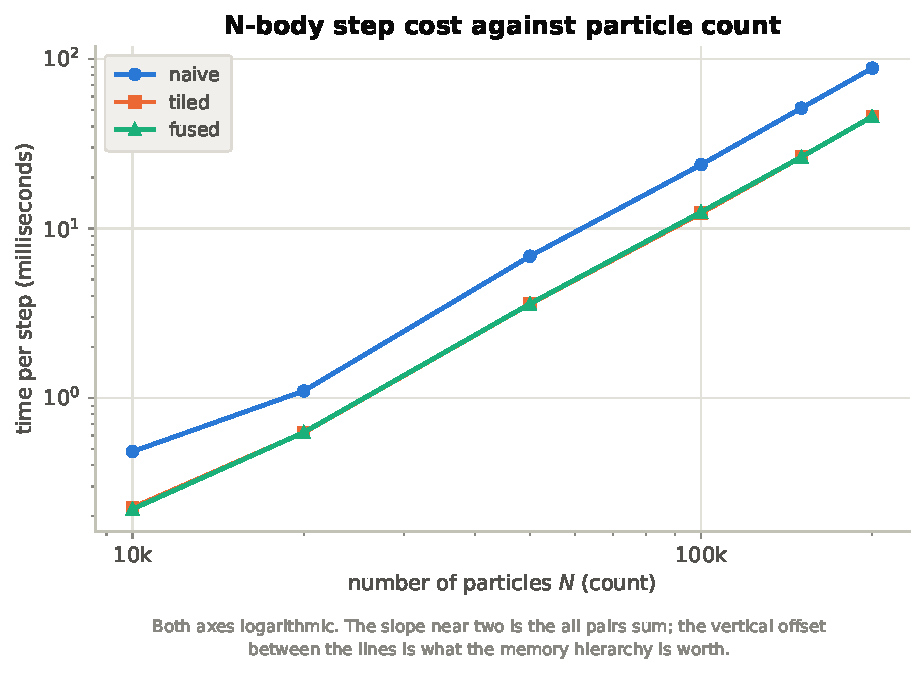
\includegraphics[width=\textwidth]{figures/fig_nbody_time}
  \caption{Step cost against particle count for the three variants.}
  \label{fig:nbodytime}
\end{figure}

\begin{figure}[htbp]
  \centering
  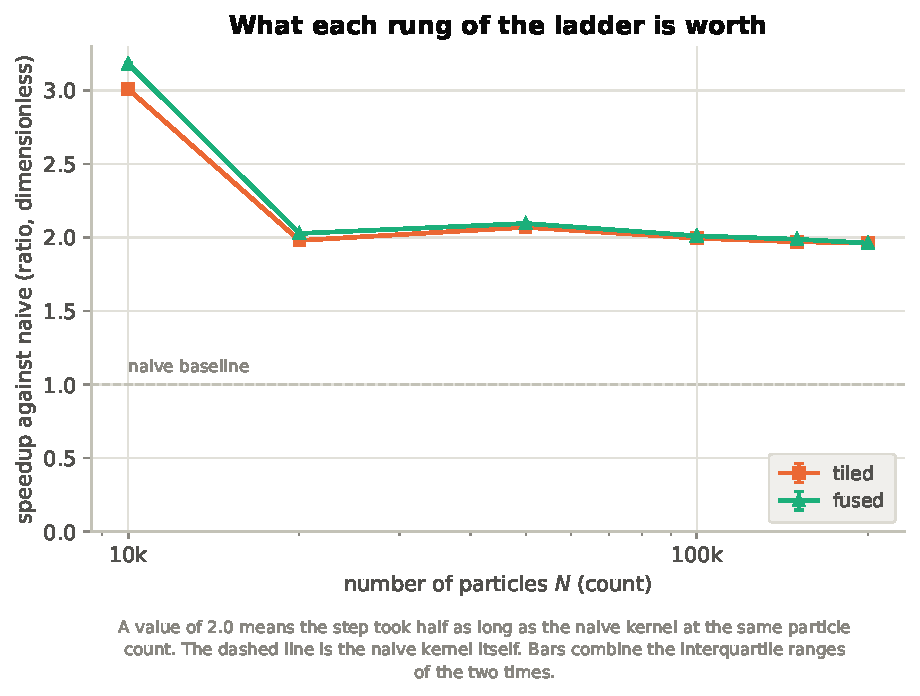
\includegraphics[width=\textwidth]{figures/fig_nbody_speedup}
  \caption{The same data as a speedup against the naive baseline. The tiled and
  fused lines lie close together; Section~\ref{sec:fusion} reads the gap between
  them.}
  \label{fig:nbodyspeedup}
\end{figure}

Tiling is worth a factor of \TilingSpeedupAtMaxN{} at \LadderMaxN{} particles,
taking the step from \NaiveMsAtMaxN{} to \TiledMsAtMaxN{} milliseconds. The paired
ratio of tiled to naive there is \TiledOverNaiveRatioAtMaxN{}, with an interquartile
range of \TiledOverNaiveRatioIqrAtMaxN{}. The factor does not grow with particle
count: it is \TilingSpeedupAtTenThousand{} at \LadderMinN{} particles and close to
two from twenty thousand up, \TilingSpeedupAtTwentyThousand{} there and
\TilingSpeedupAtMaxN{} at the largest size. \texttt{v1.0.0} said here that the
advantage grows with particle count and gave a mechanism for it, and its own table
contradicted both. I have no measurement that explains the larger factor at
\LadderMinN{}.

At the largest size the tiled kernel computes \TiledGigaInteractionsAtMaxN{} billion
pairwise interactions per second. That count is the measurement. Turning it into
floating point operations takes a convention: at the
\ConventionalFlopsPerInteraction{} operations per interaction used by Nyland, Harris
and Prins \cite{nyland2007} it is \TiledTflopsAtMaxN{} TFLOP/s, and at the
\MeasuredFlopsPerInteraction{} the hardware counters report, counting a fused multiply
add as two, it is \TiledTflopsAtMeasuredFlops{} TFLOP/s. Every TFLOP/s figure in this
report uses the convention, so it can be compared with other work that does. The peak
anywhere in the sweep is \PeakTflops{} TFLOP/s on the same basis.

\section{Fusion, expectation against measurement}
\label{sec:fusion}

Before measuring, I expected fusion to be worth ten to twenty percent. It is not
worth that at any size. Table~\ref{tab:paired} gives the fused time over the tiled
time. At \LadderMinN{} particles the ratio is \FusedOverTiledRatioAtTenThousand{},
with an interquartile range of \FusedOverTiledIqrAtTenThousand{}, and at one hundred
and fifty thousand it is \FusedOverTiledRatioAtHundredFiftyThousand{}, with a range of
\FusedOverTiledIqrAtHundredFiftyThousand{}. From \LadderMinN{} to one hundred and fifty
thousand the gain is larger than both its own interquartile range and the session
drift of \RepeatabilitySpread{} percent, so at the default tile width the fused kernel
is measurably faster, by about one percent over most of that range.

At \LadderMaxN{} particles the difference is not resolved. The ratio is
\FusedOverTiledRatioAtMaxN{} with an interquartile range of
\FusedOverTiledRatioIqrAtMaxN{}, because the tiled trials there are bimodal:
\TiledHighModeRoundsAtMaxN{} of the \PairedRoundsAtMaxN{} rounds sit near
\TiledHighModeMsAtMaxN{} milliseconds and the rest near \TiledLowModeMsAtMaxN{}. I do
not yet understand why. One hundred and fifty thousand particles shows no such split.

What fusion removes is known from the code. The split path takes three launches: half
kick and drift, force, closing half kick. Both integrator launches read the
acceleration array, $24N$ bytes per step, and the velocities are read and written
twice. The fused path takes one launch and does not read the acceleration array at
all. It still writes it, $12N$ bytes, although the engine never reads that write,
because the diagnostics and the velocity conversions recompute the force first.
Counting each array once per launch, and leaving out the repeated source reads of the
force sum, which both paths share and which dominate, the split path touches
\ModelBytesPerParticleSplit{} bytes per particle per step and the fused path
\ModelBytesPerParticleFused{}, so fusion removes \ModelBytesPerParticleSaved{}$N$ bytes
and two launches.

That traffic does not explain the gain. At the measured streaming bandwidth of
\GpuMeasuredBandwidth{} GB/s, \ModelBytesPerParticleSaved{}$N$ bytes take
\ModelSavingMsAtMaxN{} milliseconds at \LadderMaxN{} particles, which is
\ModelSavingPercentAtMaxN{} percent of a step, and \ModelSavingPercentAtMinN{} percent
at \LadderMinN{}. The measured gains are several times larger at every resolved size.
\texttt{v1.0.0} called a figure of this kind the absolute ceiling on what fusion could
deliver. It is not a ceiling: it prices one resource and says nothing about the rest
of the step. The time saved rises with particle count up to one hundred and fifty
thousand, so a fixed launch cost cannot be all of it either. The source of the gain
has not been measured.

The hardware counters do show why the expectation of ten to twenty percent was too
high.

\begin{table}[htbp]
  \centering
  \begin{tabular}{l rrr rr}
\toprule
& \multicolumn{3}{c}{throughput, percent of peak} & \multicolumn{2}{c}{per launch} \\
\cmidrule(lr){2-4}\cmidrule(lr){5-6}
variant & L1 and load store & L2 & device memory & global load sectors & warp issue \\
\midrule
naive & 87.98 & 1.62 & 0.34 & 5,000.1M & 54.99 \\
tiled & 45.41 & 1.61 & 0.35 & 78.3M & 82.68 \\
fused & 45.90 & 1.64 & 0.31 & 78.3M & 83.59 \\
\bottomrule
\end{tabular}

  \caption{Nsight Compute counters for one launch at \ProfileParticles{} particles.
  Device memory throughput is below one percent of peak for every variant.}
  \label{tab:counters}
\end{table}

Device memory throughput is \NaiveDramPct{} percent of peak for the naive kernel and
\TiledDramPct{} percent for the tiled one. The all pairs sum is $O(N^2)$ arithmetic over
$O(N)$ data, and device memory is almost idle throughout, so there was no device memory
pressure for fusion to relieve.

\section{What tiling actually fixes}

Table~\ref{tab:counters} also corrects a second assumption. Tiling is usually
described as a bandwidth optimisation, and on this problem it is not one:
device memory throughput is negligible both before and after. What tiling
reduces is pressure on the first level cache and the load store pipeline.

Global load sectors fall by a factor of \SectorReduction{} and load store
instructions by a factor of \LsuReduction{}. First level cache throughput falls
from \NaiveLoneTexPct{} percent of peak, which is close to saturation and the
highest figure in the naive row, to \TiledLoneTexPct{} percent. Warp issue
efficiency rises from \NaiveIssuePct{} percent to \TiledIssuePct{} percent. The
naive kernel's SM throughput equals its first level cache figure, and the tiled
kernel's equals its issue figure, which points at the limiting unit
of each.

The arithmetic instruction counts are the control in this experiment. They are
equal across the three variants to within a fraction of a percent, confirming
that the variants differ only in how they move data.

\begin{figure}[htbp]
  \centering
  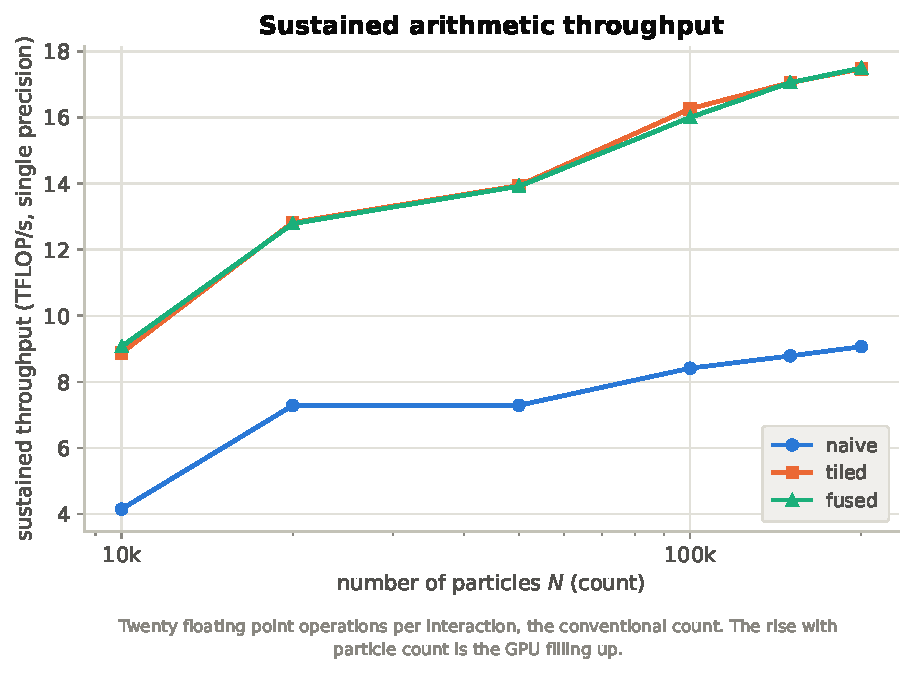
\includegraphics[width=\textwidth]{figures/fig_nbody_throughput}
  \caption{Throughput of each variant at the conventional
  \ConventionalFlopsPerInteraction{} operations per interaction.}
  \label{fig:throughput}
\end{figure}

\section{Tile width}
\label{sec:tilewidth}

\begin{table}[htbp]
  \centering
  \begin{tabular}{r rr rr}
\toprule
& \multicolumn{2}{c}{tiled} & \multicolumn{2}{c}{fused} \\
\cmidrule(lr){2-3}\cmidrule(lr){4-5}
tile width & ms per step & TFLOP/s & ms per step & TFLOP/s \\
\midrule
32 & 12.116 & 16.51 & 12.110 & 16.52 \\
64 & 11.777 & 16.98 & 11.769 & 16.99 \\
128 & 11.585 & 17.26 & 11.490 & 17.41 \\
256 & 11.487 & 17.41 & 11.373 & 17.59 \\
\bottomrule
\end{tabular}

  \caption{Tile width sweep at \TileSweepParticles{} particles. Both variants time a
  whole step.}
  \label{tab:tiles}
\end{table}

\begin{figure}[htbp]
  \centering
  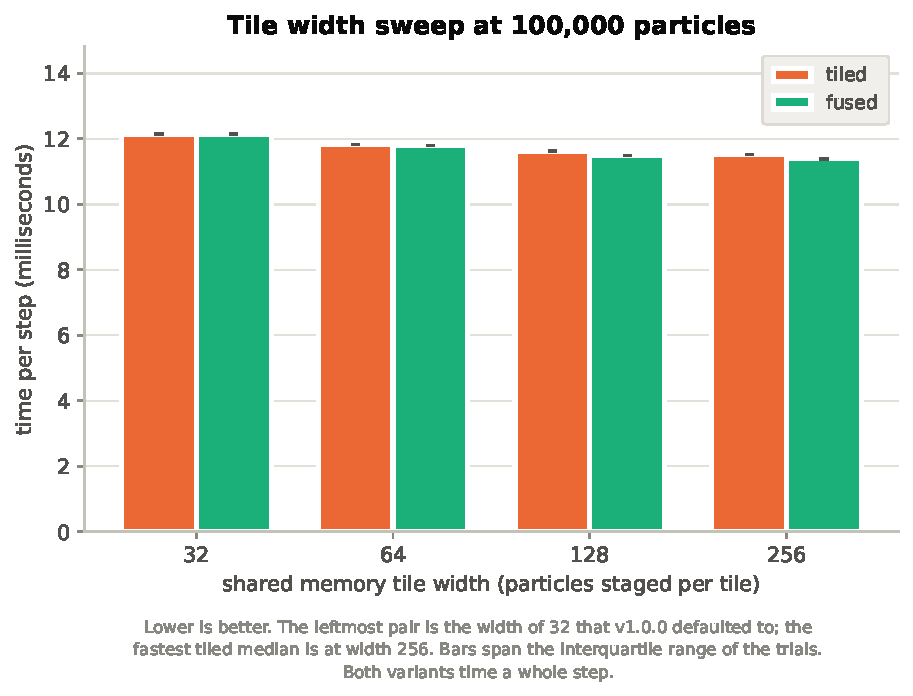
\includegraphics[width=\textwidth]{figures/fig_tile_sweep}
  \caption{Step cost against shared memory tile width.}
  \label{fig:tiles}
\end{figure}

The default tile width is now \BestTileWidth{}, the fastest of the four measured. It
runs at \BestTileMs{} milliseconds against \TileThirtyTwoMs{} for a width of thirty
two, the \texttt{v1.0.0} default, a difference of \TileWidthGainPercent{} percent. Taken
round by round the ratio is \BestTileOverTileThirtyTwoRatio{} with an interquartile
range of \BestTileOverTileThirtyTwoRatioIqr{}, well outside the session drift of
\RepeatabilitySpread{} percent. Two barriers are paid per tile, so a narrow tile pays
them more often per unit of arithmetic, which fits the direction of the result; the
barrier cost itself was not measured separately.

\section{The fluid solver}
\label{sec:sphresults}

\begin{table}[htbp]
  \centering
  \begin{tabular}{r rrr}
\toprule
particles & milliseconds per step & steps per second & million particles per second \\
\midrule
10,000 & 0.0830 & 12,049 & 120.5 \\
25,000 & 0.0969 & 10,324 & 258.1 \\
50,000 & 0.1137 & 8,794 & 439.7 \\
75,000 & 0.1537 & 6,507 & 488.0 \\
100,000 & 0.1873 & 5,338 & 533.8 \\
\bottomrule
\end{tabular}

  \caption{Fluid step cost against particle count.}
  \label{tab:sph}
\end{table}

\begin{figure}[htbp]
  \centering
  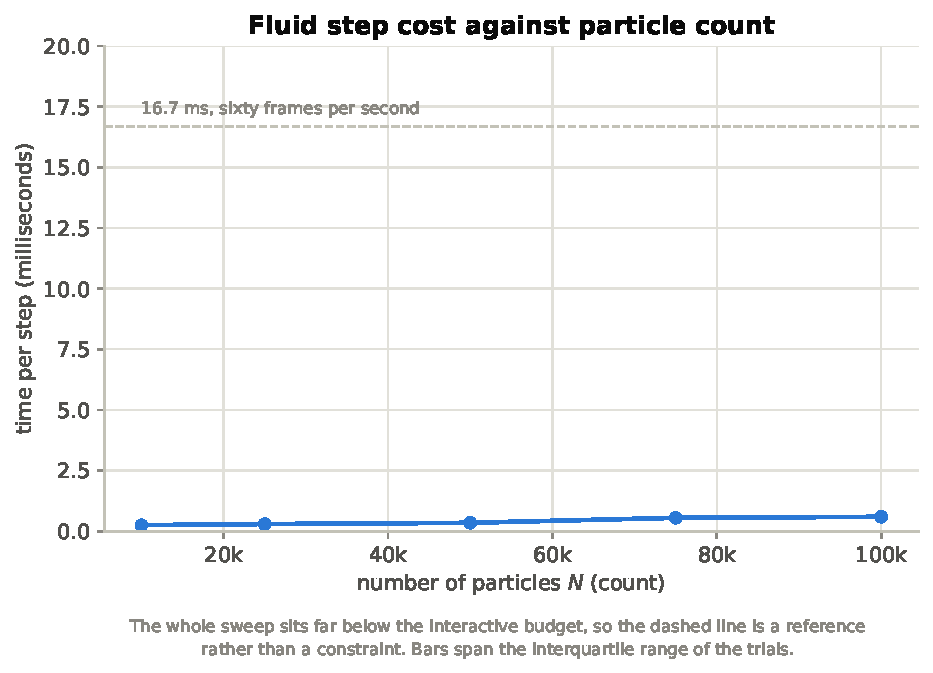
\includegraphics[width=\textwidth]{figures/fig_sph_scaling}
  \caption{Fluid step cost against particle count.}
  \label{fig:sph}
\end{figure}

At fifty thousand particles, the size of the shipped dam break, a step costs
\SphMsAtFiftyThousand{} milliseconds, or \SphFpsAtFiftyThousand{} steps per second,
which is \SphInteractiveMargin{} times inside a sixty frame per second budget. At
\SphMaxN{} particles it costs \SphMsAtMaxN{} milliseconds, \SphFpsAtMaxN{} steps per
second. These results are not comparable with \texttt{v1.0.0}, because the particle mass
changed and the fluid behaves differently.

The interquartile range of the fluid trials is \SphIqrLeastPercent{} to
\SphIqrMostPercent{} percent of the median, far above the session drift. That is the
flow rather than noise: each engine stays alive across its trials, so a size advances
through \SphTimedStepsLeast{} to \SphTimedStepsMost{} timed steps, and the per round
times trace a smooth curve as the fluid moves and its neighbour lists change.

Scaling is sublinear at the small end: \SphCountRatio{} times the particles cost
\SphTimeRatio{} times the time. A step takes six launches whatever its size, and their
fixed cost is a plausible reason, but I have not profiled the fluid step.

\section{Physics gates}
\label{sec:gates}

\begin{table}[htbp]
  \centering
  \resizebox{\textwidth}{!}{\begin{tabular}{l r r c}
\toprule
gate & measured & limit & verdict \\
\midrule
Two body orbit, relative energy drift over 10,000 steps & $1.33 \times 10^{-5}$ & $<$ 0.0010 & \textbf{pass} \\
Two body orbit, departure from circular & $9.35 \times 10^{-6}$ & $<$ 0.0010 & \textbf{pass} \\
Velocity Verlet energy order, eccentric orbit, distance of slope from 2 & 0.0072 & $<$ 0.1500 & \textbf{pass} \\
Velocity Verlet energy order, circular orbit, distance of slope from 4 & 0.0040 & $<$ 0.1500 & \textbf{pass} \\
Plummer 10k, relative momentum drift over 1,000 steps & $1.23 \times 10^{-8}$ & $<$ 0.0119 & \textbf{pass} \\
Force against a double precision CPU reference, 100 particles & $5.77 \times 10^{-7}$ & $<$ $1.00 \times 10^{-5}$ & \textbf{pass} \\
Pairwise force antisymmetry residual & $1.53 \times 10^{-7}$ & $<$ $1.00 \times 10^{-6}$ & \textbf{pass} \\
Plummer radial density, chi squared p value & 0.4416 & $>$ 0.0500 & \textbf{pass} \\
SPH poly6 kernel normalisation error & $6.48 \times 10^{-8}$ & $<$ 0.0010 & \textbf{pass} \\
SPH spiky kernel normalisation error & $4.39 \times 10^{-8}$ & $<$ 0.0010 & \textbf{pass} \\
SPH interior density, mean error & $2.81 \times 10^{-4}$ & $<$ 0.0100 & \textbf{pass} \\
SPH interior density, RMS deviation & 0.0149 & $<$ 0.0500 & \textbf{pass} \\
SPH interior density, maximum deviation & 0.0634 & $<$ 0.1000 & \textbf{pass} \\
SPH neighbour search against a brute force sum & $2.85 \times 10^{-7}$ & $<$ $1.00 \times 10^{-4}$ & \textbf{pass} \\
\bottomrule
\end{tabular}
}
  \caption{Every physics gate, its measured value and its limit. All values
  come from the artifacts written by the validation suite, which links the
  library compiled with fast math off.}
  \label{tab:gates}
\end{table}

All \GateCount{} gates pass. The margins differ widely and not all of them mean the
same thing: \texttt{docs/physics\_validation.md} classifies each as a gate, a
consistency check or a sanity check, and gives the source of its limit.

\begin{figure}[htbp]
  \centering
  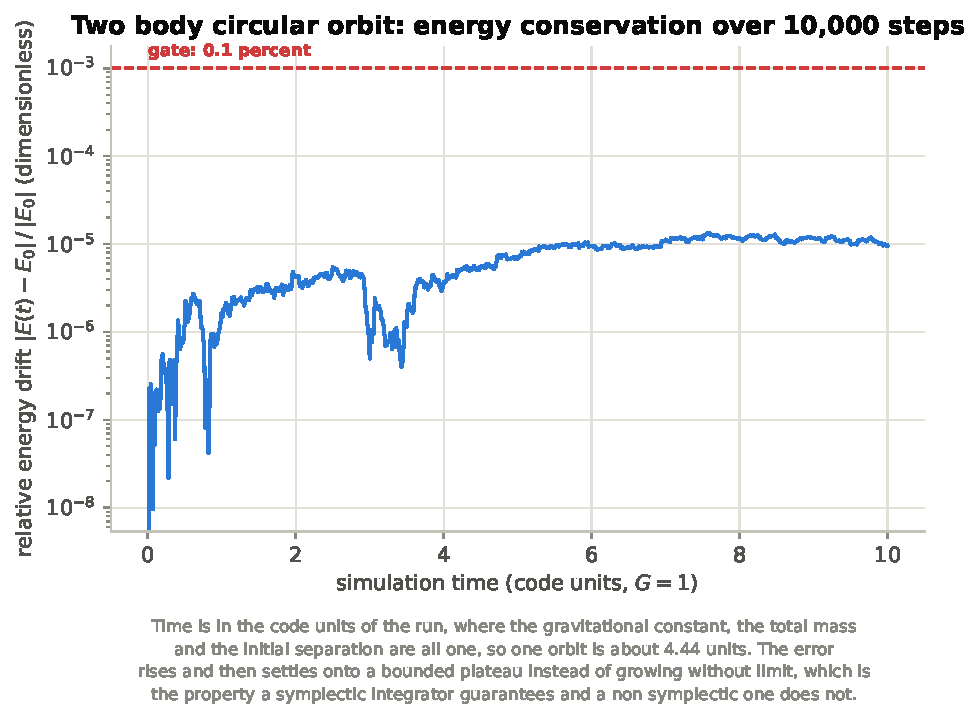
\includegraphics[width=\textwidth]{figures/fig_energy_drift}
  \caption{Relative energy error of the single precision two body orbit. At this step
  size it is single precision rounding, not integrator truncation.}
  \label{fig:energy}
\end{figure}

The two body energy error over ten thousand steps is \EnergyDriftMeasured{} against a
limit of one part in a thousand. That figure is dominated by single precision rounding:
the same orbit in double precision has a truncation error of about
$9.9 \times 10^{-13}$. So it is a regression test for the single precision path and says
nothing about the integrator's order, and the shape of
Figure~\ref{fig:energy} is the shape of rounding. \texttt{v1.0.0} read that shape as the
signature of a symplectic integrator, which it cannot show.

Order is now tested in double precision. The slope of the energy error against the time
step comes within \VerletSlopeErrorEccentric{} of two on an orbit of eccentricity 0.5,
which is the method's order, and within \VerletSlopeErrorCircular{} of four on an
unsoftened circular orbit, where symmetry cancels the second order term. Both limits were
committed before the code that measures them existed.

\begin{figure}[htbp]
  \centering
  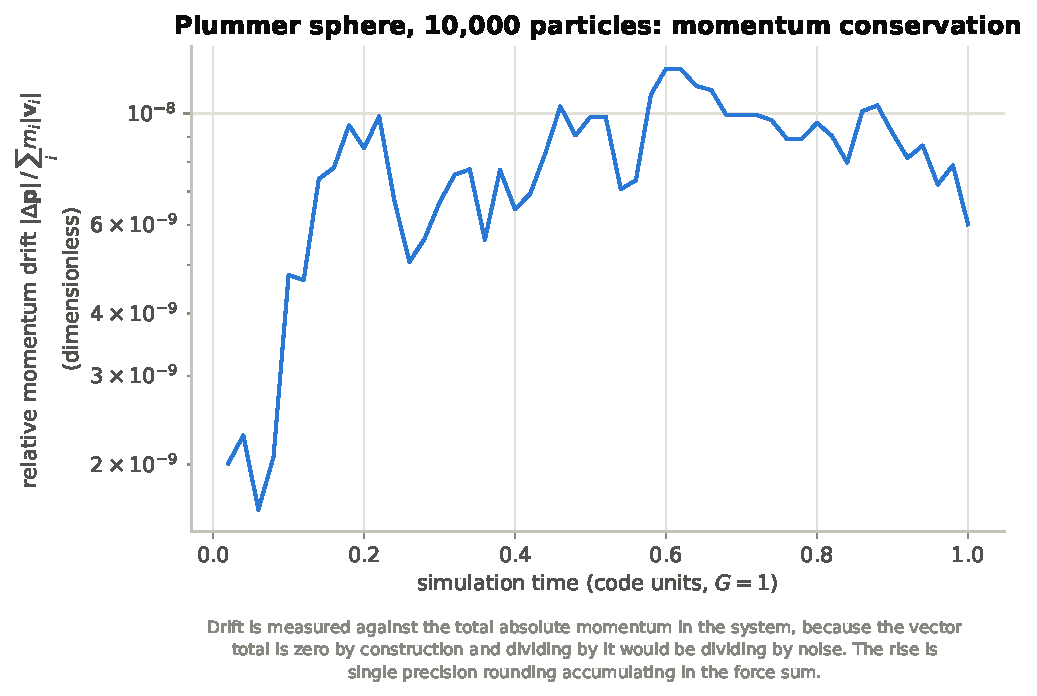
\includegraphics[width=\textwidth]{figures/fig_momentum_drift}
  \caption{Momentum conservation of a ten thousand particle Plummer sphere.}
  \label{fig:momentum}
\end{figure}

Momentum holds to \MomentumDriftMeasured{} relative to the total absolute
momentum in the system, six orders of magnitude inside the bound that single
precision arithmetic can explain. A bound that far away only rules out gross breakage.

\begin{figure}[htbp]
  \centering
  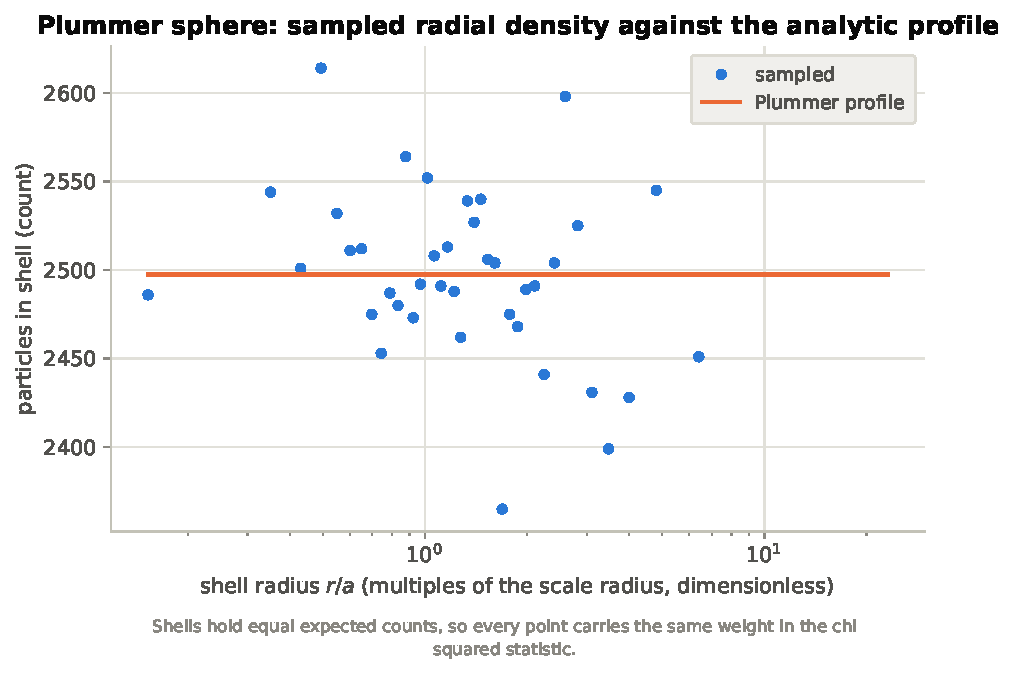
\includegraphics[width=\textwidth]{figures/fig_plummer_density}
  \caption{Sampled radial density of the Plummer sphere against the analytic
  profile.}
  \label{fig:plummer}
\end{figure}

The radial density fits the analytic profile at a chi squared p value of
\PlummerPValue{}, above the threshold of 0.05. With a fixed seed that value is a fixed
seed regression and does not vary from run to run. The same test applied to a model whose
scale radius is ten percent wrong returns a p value below $10^{-6}$, which is what
establishes that the test can reject at all.

For the fluid solver, the poly6 kernel integrates to one with an error of
\PolySixNormalisationError{}, and the density field from the hashed neighbour search
agrees with a brute force $O(N^2)$ sum over the same positions to \NeighbourSearchError{}.

The particle mass now comes from a kernel sum over the lattice actually laid out, so that
the interior of the block sits at rest density. Against that calibration the interior
mean density error is \SphDensityErrorPercent{} percent. The calibration sets this value,
so it shows the device agrees with the host calculation and is not evidence of physical
accuracy. The figures the calibration does not set are the RMS deviation of
\SphDensityRmsPercent{} percent, which lattice jitter drives, and the maximum deviation
of \SphDensityMaxPercent{} percent. Chapter~\ref{ch:corrections} records what
\texttt{v1.0.0} reported here and why it was wrong.

\chapter{Discussion}
\label{ch:discussion}

\section{The most useful result was the one that failed to appear}

The fusion measurement is the part of this project I would keep if I could keep
only one thing. The expectation of ten to twenty percent was not arbitrary; it
is roughly right for a memory bound kernel, and removing a $24N$ byte round trip
per step sounds substantial when stated in bytes. It is worth
\FusionGainPercentAtMaxN{} percent.

What the expectation missed is arithmetic intensity. The all pairs sum performs
$O(N^2)$ arithmetic on $O(N)$ data, so the ratio of operations to bytes grows
without limit as the problem grows. At \LadderMaxN{} particles the force
evaluation performs about $4 \times 10^{11}$ floating point operations while
touching a working set of a few megabytes. Removing memory traffic from a
kernel in that regime is removing something that was not costing anything: the
counters put device memory throughput at \TiledDramPct{} percent of peak.

The general lesson is that an optimisation should be sized against the resource
it relieves before it is implemented, not after. Two minutes of arithmetic with
the measured bandwidth figure would have predicted
\FusionCeilingPercent{} percent as an upper bound and saved the effort of
being surprised. That said, the fused kernel is not wasted: it is the correct
choice at small particle counts, where it wins \FusionGainPercentAtMinN{}
percent because launch overhead is then a real fraction of the step, and it
halves the memory footprint of a step.

\section{Tiling is not a bandwidth optimisation here}

The second correction is subtler. Shared memory tiling is conventionally
introduced as a way of reducing device memory traffic, and the introduction to
this report frames it that way. On this problem the framing is wrong, and the
counters say so: device memory throughput is under one percent of peak both
before and after the change. Tiling still delivers a factor of
\TilingSpeedupAtMaxN{}, but the resource it relieves is the first level cache
and the load store pipeline, not the memory bus. Global load sectors fall by a
factor of \SectorReduction{}, and the naive kernel's first level cache
throughput of \NaiveLoneTexPct{} percent of peak identifies it as the true
bottleneck.

This matters practically. Had I tried to improve the naive kernel by attacking
device memory traffic, for instance by compressing the state or by adding
prefetching, nothing would have happened. The profile pointed at the right
resource; reasoning from the textbook description would not have.

\section{Where the specification and the measurement disagreed}

Three points in the original design were changed or contradicted by
measurement, and each is recorded rather than quietly absorbed.

The host compiler floor of GCC 16.1 is not achievable with CUDA 13.3, which
refuses any GCC newer than 15. GCC 15.2 supplies the C++23 host standard the
floor was really for.

The tile width of thirty two costs \TileWidthGainPercent{} percent against a
width of \BestTileWidth{} on this card. The default was kept so the ladder
would measure the design as specified, and the sweep is reported so the choice
is informed.

The estimated runtimes in the specification are far too long. The full
validation suite, which was estimated at ten to twenty minutes on the grounds
that the ten thousand step orbit would dominate, completes in about five
seconds. The estimate assumed the orbit run would be expensive; with two
particles it is trivially cheap, and the cost is dominated instead by the ten
thousand particle Plummer runs. The full benchmark sweep, estimated at fifteen
to thirty minutes, completes in under two minutes.

\section{Limitations}

The all pairs solver is $O(N^2)$ and always will be. At two hundred thousand
particles a step costs \TiledMsAtMaxN{} milliseconds; at two million it would
cost a hundred times that. The range where this approach is the right one is
bounded, and beyond it a tree code is not an optimisation but a different
algorithm.

The fluid solver is weakly compressible, so it enforces incompressibility only
through a stiff equation of state. That bounds the time step: the sound speed
implied by the stiffness constant sets a Courant condition far tighter than the
fluid velocity would. The dam break runs at a time step of $10^{-4}$ seconds
for that reason, so the interactive step rates reported in
Section~\ref{sec:sphresults} are steps per second and not seconds of simulated
time per second.

Single precision is a deliberate choice and it has a cost. The momentum gate
measures it directly: the residual is exactly the accumulation of rounding in
the force sum. For the problems here that cost is far inside the tolerances,
but a long term integration of a planetary system would need double precision
positions, and the ladder would look different because double precision
arithmetic is much slower relative to memory on consumer hardware.

The benchmark measures the fluid from a configuration that begins as a settled
block and evolves for a few hundred steps during measurement. A fully developed
splash has a different spatial distribution and therefore a different neighbour
list length, so the fluid timings should be read as representative of the early
collapse rather than of every phase of the flow.

\chapter{Conclusion}
\label{ch:conclusion}

The engine does what it was built to do. Direct N-body gravity runs at
\TiledTflopsAtMaxN{} TFLOP/s of sustained single precision arithmetic at
\LadderMaxN{} particles, and the fluid solver runs \SphMaxN{} particles at
\SphMsAtMaxN{} milliseconds per step, roughly fifty times inside an interactive
budget at the fifty thousand particles it was aimed at. All \GateCount{}
physics gates pass, most with orders of magnitude of margin, against a library
compiled with fast math disabled so that no compiler flag can relax them.

The memory hierarchy ladder produced a clear answer and a clear correction.
Shared memory tiling is worth a factor of \TilingSpeedupAtMaxN{}, and the
hardware counters attribute that gain to a \SectorReduction{} times reduction
in global load sectors relieving a saturated load store pipeline, not to device
memory bandwidth, which never rose above one percent of peak in any variant.
Fusing the integrator into the force kernel was expected to be worth ten to
twenty percent and is worth \FusionGainPercentAtMaxN{} percent, for the good
reason that an $O(N^2)$ arithmetic problem on $O(N)$ data is not waiting on
memory at all. Both results are more useful than the numbers I expected to
report, because both changed how I would size the next optimisation before
writing it.

The parts of the design that survived contact with measurement did so because
they were chosen against a specific failure. Velocity Verlet was chosen because
its energy error is bounded rather than merely small, and
Figure~\ref{fig:energy} shows exactly that shape. The exact cell key comparison
in the neighbour search was added because hashing is many to one and a bucket
scan would otherwise count some neighbours twice, and the brute force
comparison confirms it works to three parts in ten million. Double precision
diagnostic accumulators were chosen because a single precision reduction would
have measured itself rather than the integrator.

\section{Further work}

A Barnes Hut tree code is the obvious next step and the one that changes the
reachable problem size rather than the constant factor. Its irregular traversal
is a genuinely different GPU problem, and the tiled kernel here would remain the
right choice for the leaf level interactions.

The fluid solver would benefit more from a position based or projection based
incompressibility treatment than from any further kernel tuning, because the
stiff equation of state, not the neighbour search, is what bounds the time step.

The tile width result suggests a small piece of unfinished business: with the
default at thirty two for fidelity to the specification, and \BestTileWidth{}
measurably faster, the right resolution is to make the width a configuration
field so the ladder can be run at the specified width while production runs use
the fastest one.


\bibliographystyle{plain}
\bibliography{refs}

\end{document}
